\documentclass{article}
\usepackage{multicol}
\usepackage{booktabs} 
\usepackage{blindtext}
\usepackage{float}  


\renewcommand{\refname}{Referencias}
\renewcommand{\tablename}{Tabla}

\title{Ejemplo de Documento Sweave}
\author{Carlos Schmidt}
\date{2024-07-22}

\usepackage{Sweave}
\begin{document}
\Sconcordance{concordance:Ejemplo.tex:Ejemplo.Rnw:1 12 1 1 0 15 1 1 8 1 5 6 1 1 30 19 %
1 1 35 1 2 6 1 1 27 18 1 1 36 1 2 6 1 1 27 17 1 1 45 1 2 38 1}


\maketitle

\textbf{Preguntas a las que este informe da respuesta:}
\begin{enumerate}
    \item ¿Cómo varían las tres motivaciones contempladas (extrínseca, intrínseca y prosocial) en función del sexo de los sujetos?
    \item ¿Cómo varían las tres motivaciones contempladas (extrínseca, intrínseca y prosocial) en función de la edad de los sujetos?
    \item ¿Cómo varían las tres motivaciones contempladas (extrínseca, intrínseca y prosocial) en función del nivel educativo de los sujetos?
    \item ¿Cuál es la distribución de los niveles de las tres motivaciones contempladas (extrínseca, intrínseca y prosocial) en los países de Europa occidental?
    \item ¿Cuál es la motivación principal de entre las tres contempladas (extrínseca, intrínseca y prosocial) en los países de Europa occidental?
\end{enumerate}





\section{Pregunta: ¿Cómo varían las tres motivaciones contempladas (extrínseca, intrínseca y prosocial) en función del sexo de los sujetos?
}

En esta sección, comentamos el resultado de un t-test realizado para comparar las medias de la motivación intrínseca, extrínseca y prosocial por género.


Los resultados del t-test indican que hay diferencias estadísticamente significativas entre las medias de hombres y mujeres en las tres motivaciones contempladas. En concreto: las medias de las mujeres en motivación extrínseca (3.78) y motivación intrínseca (3.19) son más altas que las de los hombres (3.56 y 3.02), y la de los hombres lo es en motivación prosocial (2.01 frente a 1.85).

\begin{table}[h!]
\centering
\caption{Resultados del t-test para cada motivación por género}
\begin{tabular}{lccc}
  \toprule
  \textbf{Motivación} & \textbf{Media Hombres} & \textbf{Media Mujeres} & \textbf{p-valor} \\
  \midrule
  Motivación Prosocial & 2.01 & 1.85 & 0 \\
  Motivación Extrínseca & 3.56 & 3.78 & 0 \\
  Motivación Intrínseca & 3.02 & 3.19 & 0 \\
  \bottomrule
\end{tabular}
\end{table}


\subsection{Gráfico de motivaciones por sexo}

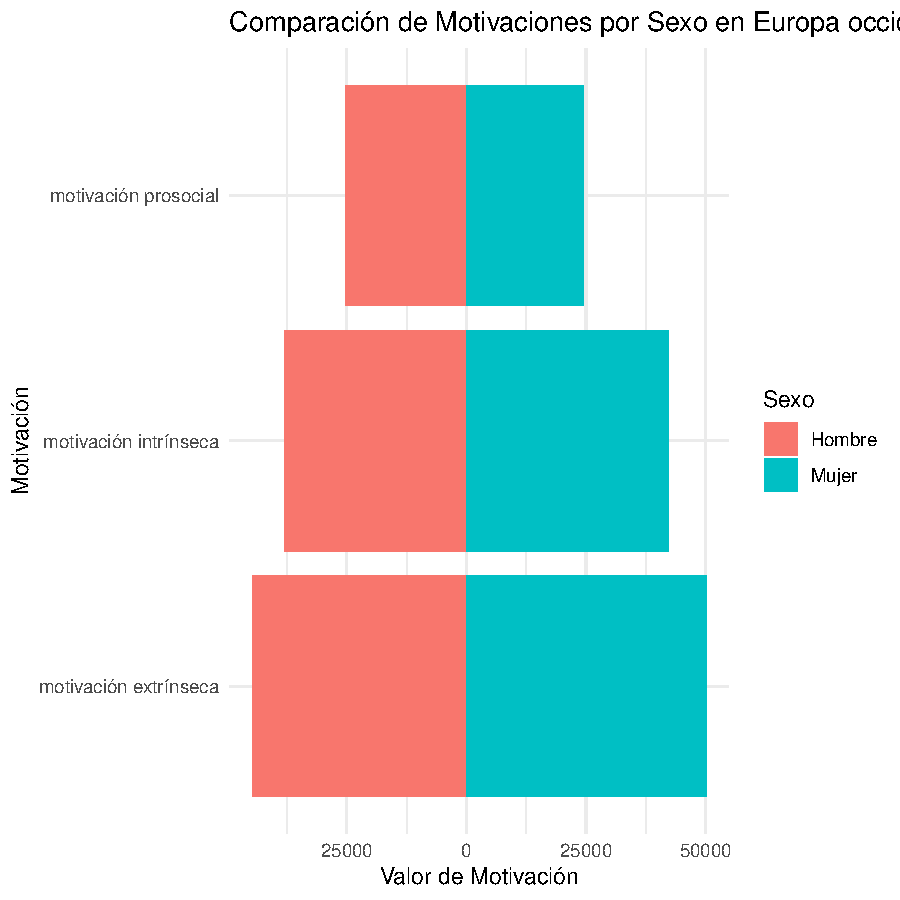
\includegraphics{Ejemplo-004}



\section{Pregunta: ¿Cómo varían las tres motivaciones contempladas (extrínseca, intrínseca y prosocial) en función de la edad de los sujetos?}

En esta sección, realizaremos ANOVAs para comparar las medias de la motivación intrínseca, extrínseca y prosocial por categorías de edad.


Los resultados de los ANOVAs indican que las diferencias entre las medias de la motivación prosocial según las categorías de edad son significativas (F(7, 25819) = 2.492, p = 0.0148). Indican que las diferencias entre las medias de la motivación extrínseca según las categorías de edad son significativas (F(7, 25819) = 282.1, p < 0.00e+00)., e indican también que las diferencias entre las medias de la motivación intrínseca según las categorías de edad son asimismo significativas (F(7, 25819) = 366.4, p < 0.00e+00).

\begin{table}[h!]
\centering
\caption{Resultados del ANOVA para cada motivación por categoría de edad}
\begin{tabular}{lcc}
  \toprule
  \textbf{Motivación} & \textbf{F-valor} & \textbf{p-valor} \\
  \midrule
  Motivación Prosocial & 2.492 & 0.0148 \\
  Motivación Extrínseca & 282.1 & 0.00e+00 \\
  Motivación Intrínseca & 366.4 & 0.00e+00 \\
  \bottomrule
\end{tabular}
\end{table}


\subsection{Gráfico de motivaciones por edad}
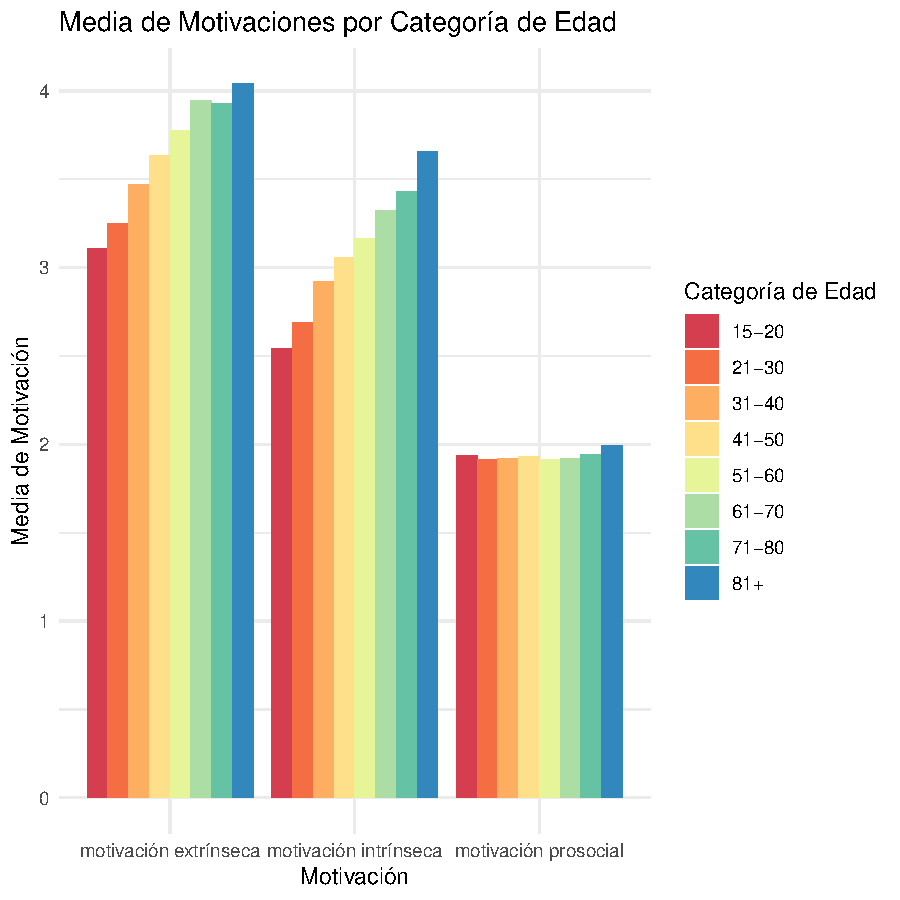
\includegraphics{Ejemplo-006}



\section{Pregunta: ¿Cómo varían las tres motivaciones contempladas (extrínseca, intrínseca y prosocial) en función del nivel educativo de los sujetos?}

En esta sección, realizamos ANOVAs para comparar las medias de la motivación intrínseca, extrínseca y prosocial por nivel educativo.


Los resultados de los ANOVAs indican que hay una diferencia significativa en la motivación prosocial entre los diferentes niveles educativos (F(3, 25823) = 32.08, p < 1.10e-20). Indican que hay diferencias significativas entre los niveles educativos en motivación extrínseca (F(3, 25823) = 25.62, p < 1.53e-16) y, asimismo, que hay una diferencia significativa entre los niveles educativos en motivación intrínseca (F(3, 25823) = 59.8, p < 1.61e-38).

\begin{table}[h!]
\centering
\caption{Resultados del ANOVA para cada motivación por nivel educativo}
\begin{tabular}{lcc}
  \toprule
  \textbf{Motivación} & \textbf{F-valor} & \textbf{p-valor} \\
  \midrule
  Motivación Prosocial & 32.08 & 1.10e-20 \\
  Motivación Extrínseca & 25.62 & 1.53e-16 \\
  Motivación Intrínseca & 59.8 & 1.61e-38 \\
  \bottomrule
\end{tabular}
\end{table}

\subsection{Gráfico de motivaciones por nivel educativo}
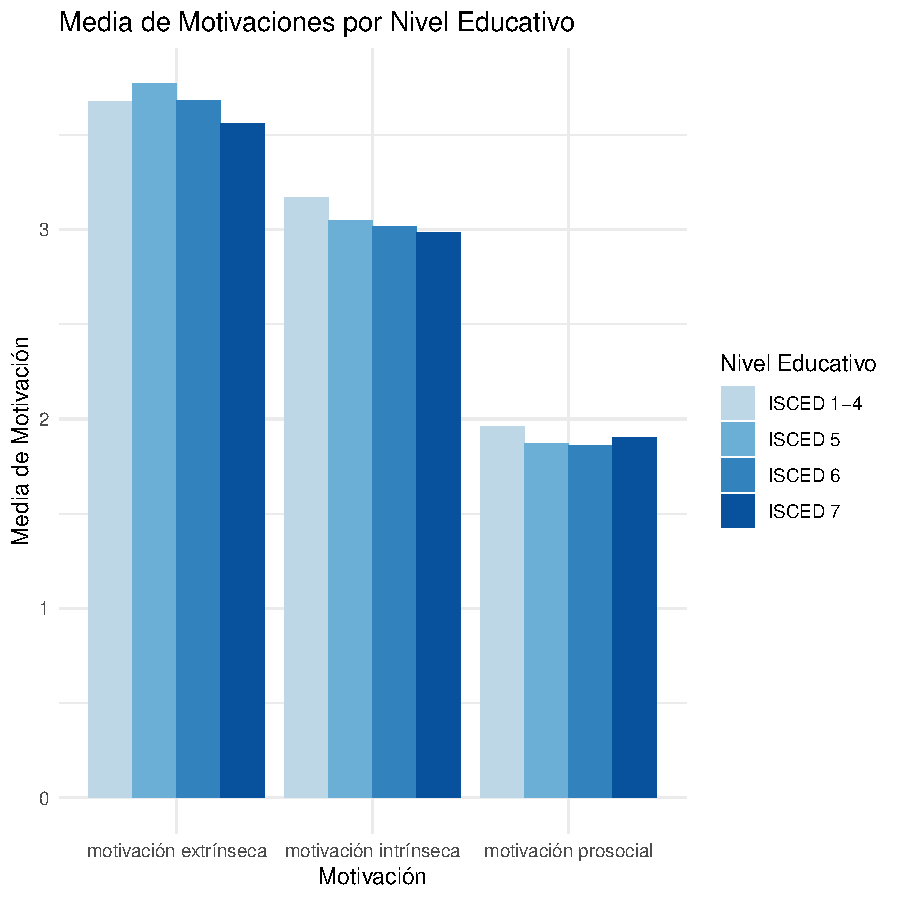
\includegraphics{Ejemplo-008}



\section {Pregunta: ¿Cuál es la distribución de los niveles de las tres motivaciones contempladas (extrínseca, intrínseca y prosocial) en los países de Europa occidental?}

En esta sección, presentamos la respuesta mediante una tabla.
Como se puede observar, todos los países menos Italia muestran la motivación extrínseca como el tipo de motivación de media más alta. EN el caso de Italia, la motivación de mayor media es la intrínseca.

\begin{table}

\caption{Media de las motivaciones por país}
\centering
\begin{tabular}[t]{lrrr}
\toprule
cntry & mean\_Prosocial & mean\_Extrínseca & mean\_Intrínseca\\
\midrule
AT & 1.83 & 3.30 & 3.02\\
BE & 1.93 & 3.42 & 2.94\\
CH & 1.78 & 3.52 & 2.72\\
DE & 1.82 & 3.76 & 3.04\\
DK & 1.80 & 3.67 & 2.78\\
\addlinespace
ES & 1.78 & 3.81 & 3.10\\
FI & 1.81 & 4.08 & 3.15\\
FR & 2.03 & 4.23 & 3.05\\
GB & 1.93 & 3.76 & 3.28\\
IE & 1.93 & 3.66 & 3.24\\
\addlinespace
IT & 2.17 & 3.09 & 3.54\\
NL & 2.02 & 3.56 & 3.04\\
NO & 2.05 & 3.89 & 3.16\\
PT & 2.08 & 3.75 & 3.17\\
SE & 1.98 & 4.04 & 3.08\\
\bottomrule
\end{tabular}
\end{table}





\section {Pregunta: ¿Cuál es la motivación principal de entre las tres contempladas (extrínseca, intrínseca y prosocial) en los países de Europa occidental?}










\end{document}

\begin{Schunk}
\begin{Sinput}
> 
\end{Sinput}
\end{Schunk}

